 %!TEX root = ./template-skripsi.tex
%-------------------------------------------------------------------------------
%                            BAB II
%               KAJIAN TEORI
%-------------------------------------------------------------------------------

\chapter{KAJIAN PUSTAKA} 

\section{Definisi \emph{Search Engine}}

\emph{Search engine} merupakan program yang memungkinkan pengguna untuk mengajukan pertanyaan atau menggunakan kata kunci untuk membantu mencari informasi di web~\cite{william2001using}. \emph{Search engine} pada dasarnya merupakan sebuah halaman web, tetapi perannya berfokus untuk mengumpulkan dan mengorganisir berbagai informasi di internet.

\section{Sejarah \emph{Search Engine}}

Mesin pencari pertama bernama \emph{Archie} atau disebut "\emph{archive}" tanpa menyebut huruf "v" yang dibuat 1990. Alan Emtage, Bill Heelan, dan J.Peter Deutsch merupakan mahasiswa ilmu komputer Universitas McGill di Montreal Kanada, mereka bersama-sama membuat mesin pencari ini. Database \emph{Archie} terdiri dari direktori file yang berisi ratusan sistem. \emph{Archie} tidak dapat mengindeks isi konten dari sebuah situs. Melainkan, \emph{Archie} secara berkala menjangkau semua situs \emph{File Transfer Protocol} (FTP) yang tersedia, kemudian membuat daftar-daftar file dan membuat indeks yang dapat dicari. Perintah untuk mencari di \emph{Archie} menggunakan perintah \emph{UNIX}, dan dibutuhkan pengetahuan tentang \emph{UNIX} untuk menggunakannya secara maksimal \cite{seymour2011history}.

Tahun 1991 muncul aplikasi bernama \emph{Gopher}. Kemunculan \emph{Gopher} membawa dua program pencarian bernama \emph{Veronica} dan \emph{Jughead}. Sama seperti \emph{Archie}, \emph{Veronica} dan \emph{Jughead} mencari nama file dan judul yang tersimpan dalam sistem indeks \emph{Gopher}. \emph{Gopher} dibuat oleh Mark McCahill pada tahun 1991 di Universitas Minnesota. \emph{Gopher} dirancang untuk mendistribusikan, mencari, dan mengambil dokumen melalui Internet. \emph{Gopher} menawarkan beberapa fitur yang tidak didukung oleh Web dan menerapkan hierarki yang lebih kuat pada informasi yang disimpan di dalamnya. \emph{Gopher} adalah sistem protokol, yang mendahului \emph{World Wide Web}, memungkinkan \emph{file} teks berbasis server diatur secara hierarki dan mudah dilihat oleh pengguna yang mengakses server menggunakan Aplikasi \emph{Gopher} di komputer jarak jauh. Awalnya Browser \emph{Gopher} hanya dapat menampilkan \emph{file} berbasis teks, kemudian terdapat pengembangan seperti \emph{Hyper Gopher} yang mampu menangani format grafik sederhana \cite{seymour2011history}.

Setelah mesin pencari pertama muncul di tahun 1990, tiga tahun berikutnya di tahun 1993 pada bulan November, muncul mesin pencari bernama \emph{Aliweb}. Mesin pencari kedua ini tidak menggunakan \emph{web robot}, dan mengizinkan pengguna untuk mengirimkan lokasi file indeks di situs mereka yang memungkinkan mesin pencari untuk memasukkan Halaman Web dan menambahkan deskripsi halaman dan kata kunci yang ditulis pengguna. \emph{Aliweb} tidak secara otomatis mengindeks situs, Jika pengguna ingin sebuah situs terindeks pada mesin pencari ini, maka pengguna harus menulis file khusus dan mendaftarkannya ke \emph{Aliweb Server} \cite{seymour2011history}.

\emph{Jumpstation} yang dirilis bulan Desember tahun 1993 menggunakan \emph{web robot} untuk mencari halaman-halaman web dan untuk membangun indeksnya. \emph{Jumpstation} adalah tool pertama yang menggunakan tiga fitur penting dari \emph{web search engine}, yaitu \emph{crawling}, \emph{indexing}, dan \emph{searching}. Karena sumberdaya pada platformnya yang terbatas, pengindeksan dan pencariannya dibatasi pada judul dan \emph{headings} yang ditemukan di halaman web oleh \emph{crawler} \cite{seymour2011history}.

\emph{Search engine} pertama yang menyediakan pencarian teks lengkap adalah \emph{WebCrawler}. \emph{Search engine} berbasis \emph{crawler} ini muncul pada tanggal 20 April 1994 dan dibuat oleh Brian Pinkerton di Universitas Washington \cite{seymour2011history}. Para pengguna dapat mencari setiap kata yang terdapat pada halaman web, dan ini menjadi standar utama pada search engine sejak saat itu.

Banyak \emph{search engine} yang kemudian muncul dan bersaing untuk memperebutkan popularitas. Beberapa diantaranya \emph{Magelan search engine}, \emph{Excite}, \emph{Infoseek}, \emph{Inktomi}, \emph{Northern Light}, dan \emph{Altavista}. \emph{Yahoo!} adalah salah satu cara yang paling populer untuk menemukan halaman web yang ingin dicari, tetapi fungsi pencariannya beroperasi pada direktori web \emph{Yahoo!}, bukan salinan teks lengkap dari halaman web.

\emph{AltaVista} pernah menjadi salah satu \emph{search engine} paling populer, muncul pada tahun 1995. Louis Monier yang memegang \emph{crawler} dan Michael Burrows yang menulis pengindeksnya. \emph{AltaVista} memiliki server komputasi yang paling kuat, dan membuat \emph{AltaVista} menjadi \emph{search engine} tercepat dan dapat menangani jutaan hit dalam sehari. Satu fitur pada \emph{AltaVista} yang menarik dibandingkan \emph{search engine} sebelumnya, yaitu pengguna dapat mengetikkan frasa atau pertanyaan, dan mendapatkan respon yang sesuai. Tetapi popularitas \emph{AltaVista} berkurang dengan munculnya \emph{Google}.

\emph{Ask Jeeves} (\emph{Ask}) adalah \emph{searh engine} yang didirikan tahun 1996 oleh Garrett Gruener dan David Warthen di Barkeley, Calivornia \cite{seymour2011history}. Ide awal kemunculan \emph{Ask} adalah untuk memudahkan pengguna mendapatkan jawaban atas pertanyaan yang diajukan dalam bahasa sehari-hari. \emph{Ask.com} saat ini masih tersedia, dengan fitur tambahan yaitu dapat menerima pertanyaan matematika, kamus, dan pertanyaan konversi.

Perusahaan \emph{Netscape} di tahun 1996 ingin memberikan kesepakatan ekslusif kepada satu \emph{search engine} untuk menjadi \emph{search engine} utama di \emph{web browser Netscape}. Keputusan yang di ambil \emph{Netscape} saat itu terdapat lima \emph{search engine} utama, dan setiap \emph{search engine} mendapat bayaran lima juta dolar per tahun. Lima \emph{search engine} tersebut adalah \emph{Yahoo!}, \emph{Magellan}, \emph{Lycos}, \emph{Infoseek}, dan \emph{Excite} \cite{seymour2011history}.

\emph{Google} resmi muncul pada tahun 1998 oleh Larry Page dan Sergey Brin, mahasiswa Universitas Stanford di California. Untuk meningkatkan hasil kualitas penelusuran, Brin dan Page memperkenalkan PageRank, sebuah metode untuk menghitung peringkat setiap halaman web \cite{page1999pagerank}. \emph{Google search engine} telah meminimalisir hasil penelusuran sampah di hasil penelusuran teratas, memudahkan pengguna untuk mencari informasi yang ada di web. Mulai sekitar tahun 2000, \emph{Google search engine} menjadi terkenal hingga saat ini. 

\emph{Yahoo!} menggunakan \emph{Google search} hingga tahun 2004, dan setelah itu membangun \emph{search engine} sendiri. Sebelumnya, \emph{Yahoo!} membeli \emph{Overture} yang memiliki \emph{search engine AlthaWeb} dan \emph{AltaVista}, walaupun memiliki banyak \emph{search engine}, \emph{Yahoo!} tidak menggunakannya untuk situs web utama \emph{yahoo.com}, menggunakan \emph{Google search} untuk hasil penelusurannya. \emph{Yahoo!} \emph{search} menggabungkan kemampuan semua perusahaan \emph{search engine} yang mereka peroleh, dan dengan penelitian yang ada, kemudian menggabungkannya kedalam satu \emph{search engine}.

\emph{Microsoft} pertama kali meluncurkan \emph{MSN search} tahun 1998, menggunakan hasil pencarian dari \emph{Inktomi} \cite{seymour2011history}. Pada tahun 2004, \emph{Microsoft} mulai transisi ke teknologi \emph{search engine} sendiri, yang didukung oleh \emph{web crawler} milik \emph{Microsoft}, bernama \emph{msnbot}. \emph{Search engine Microsoft}, yaitu \emph{Bing}, resmi diluncurkan pada tanggal 1 Juni 2009. Kemudian satu bulan lebih setelahnya tanggal 29 Juli 2009, \emph{Yahoo!} dan \emph{Microsoft} menyelesaikan kesepakatan, \emph{Yahoo!} search akan didukung oleh teknologi \emph{Microsoft Bing}.

\section{Arsitektur \emph{Search Engine}}

\emph{Search engine} bekerja dengan cara menyimpan semua informasi dari berbagai halaman web. Halaman-halaman tersebut diambil menggunakan program khusus yang disebut \emph{Web Crawler}, isi dari setiap halaman kemudian dianalisis untuk menentukan bagaimana halaman tersebut akan diindeks. Gambar \ref{gambar:google_architecture} merupakan \emph{High Level Google Architecture} \cite{brin1998anatomy}.

\begin{figure}[H]
	\centering
	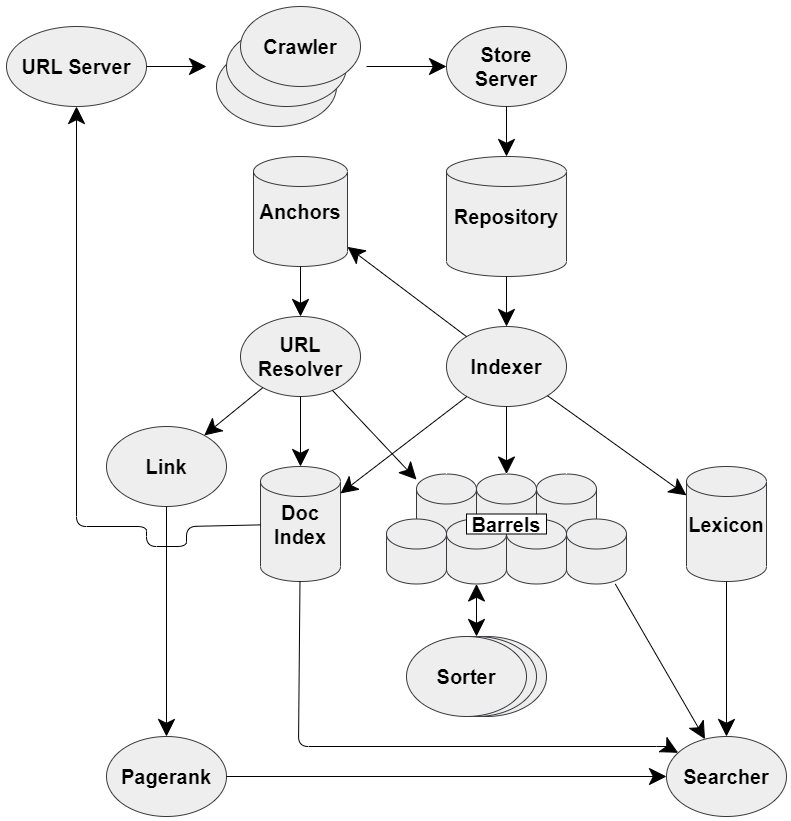
\includegraphics[keepaspectratio, width=10cm]{gambar/google_architecture}
	\caption{\emph{High Level Google Architecture} \cite{brin1998anatomy}}
	\label{gambar:google_architecture}
\end{figure}

\emph{Web crawling} (mengunduh halaman web) dilakukan oleh beberapa \emph{crawler} yang terdistribusi. Terdapat \emph{URL server} yang mengirimkan daftar \emph{URL} untuk diambil ke \emph{crawler}. Halaman web yang telah diambil kemudian dikirim ke \emph{store server} dan \emph{store server} menyimpan halaman web ke dalam \emph{Repository}. Setiap halaman web memiliki nomor ID yang disebut \emph{docID}, ditetapkan setiap kali \emph{URL} baru diurai dari halaman web. Pengindeksan dilakukan oleh \emph{indexer} dan \emph{sorter}. Fungsi dari \emph{indexer} yaitu: membaca repositori, membuka kompresi dokumen, dan mengurainya. Setiap dokumen kemudian diubah menjadi sekumpulan kejadian kata yang disebut \emph{hits}. \emph{Hits} berfungsi untuk merekam kata, menyimpan posisi dalam dokumen, menyimpan perkiraan ukuran \emph{font} dan kapitalisasi. \emph{Indexer} mendistribusikan \emph{hits} ke dalam satu set "\emph{barrels}", membuat \emph{forward index} yang diurutkan sebagian. \emph{Indexer} melakukan fungsi penting lainnya, yaitu mengurai semua \emph{link} di setiap halaman web dan menyimpan informasi penting ke dalam \emph{anchors file}. \emph{File} ini berisi informasi yang cukup untuk menentukan darimana dan kemana setiap \emph{link point}, dan berisi teks dari setiap \emph{link}.

\emph{URL resolver} membaca \emph{anchors file} dan mengubah \emph{URL} relatif menjadi \emph{URL} absolut, serta merubahnya menjadi \emph{docID}. Kemudian menempatkan \emph{anchors text} ke \emph{forward index}, terkait dengan \emph{docID} yang ditunjukkan oleh \emph{anchor}. Dan juga menghasilkan \emph{database of links} yang merupakan pasangan \emph{docID}. \emph{Database link} digunakan untuk menghitung \emph{PageRank} untuk semua dokumen.

\emph{Sorter} mengambil \emph{barrels} yang telah diurutkan berdasarkan \emph{docID} dan menggunakan \emph{barrels} dengan \emph{wordID} untuk menghasilkan \emph{inverted index}. Hal ini dilakukan di dalam sebuah tempat, sehingga sedikit ruang sementara yang dibutuhkan untuk operasi ini. \emph{Sorter} juga menghasilkan daftar \emph{wordID} dan \emph{offset} ke dalam \emph{inverted index}. Sebuah program bernama \emph{DumpLexicon} mengambil daftar \emph{wordID} bersama dengan \emph{leksicon} yang dihasilkan oleh \emph{indexer} dan menghasilkan \emph{leksicon} baru untuk digunakan oleh \emph{searcher}. \emph{Searcher} dijalankan oleh \emph{web server} dan menggunakan \emph{leksicon} yang dibuat oleh \emph{DumpLexicon} bersama dengan \emph{inverted index} dan \emph{PageRank} untuk menjawab pertanyaan.

Pada tahun 1998, \emph{Google} menjalankan proses tersebut membutuhkan waktu kurang lebih 9 hari untuk menngunduh data dari 26 juta halaman web. Jika dihitung dalam detik, maka membutuhkan waktu rata-rata sekitar 33,44 halaman per detik. Proses ini selalu diulang untuk mendapat perubahan informasi atau data yang ada di seluruh halaman web. Diimplementasikan hampir seluruhnya menggunakan \emph{C} atau \emph{C++}, tetapi sebagian lainnya, seperti \emph{URL server} dan \emph{crawler} diimplementasikan menggunakan \emph{python}.

\section{\emph{Web Crawler}}

\emph{Crawler} adalah program yang mengambil halaman Web, biasanya untuk digunakan oleh mesin pencari \cite{pinkerton1994finding}. Secara kasar, \emph{crawler} memulai dengan \emph{URL} untuk halaman awal $P_{0}$. Kemudian \emph{Crawler} mengambil $P_{0}$, mengekstrak semua \emph{URL} yang terdapat di dalam $P_{0}$, dan menambahkannya ke antrian \emph{URL} untuk dipindai. Kemudian \emph{crawler} mengambil \emph{URL} dari antrian (dalam urutan tertentu), dan mengulangi prosesnya \cite{cho1998efficient}.

\subsection{\emph{Importance Metrics}}

Tidak semua halaman memiliki minat yang sama dengan \emph{crawler's client}. Misalnya, jika \emph{client} sedang membangun database khusus tentang topik tertentu, maka halaman yang merujuk ke topik tersebut lebih penting, dan harus dikunjungi sesegera mungkin. Demikian pula, \emph{search engine} dapat menggunakan jumlah \emph{URL} Web yang mengarah ke sebuah halaman, disebut \emph{backlink count}, untuk menentukan peringkat hasil \emph{query} pengguna.

Sebuah \emph{Web page} $P$, dapat ditentukan \emph{importance of the page} $I(P)$ dengan salah satu cara berikut (Cara tersebut dapat dikombinasikan satu sama lain):

\begin{enumerate}
	\item \emph{Similarity to a Driving Query $Q$}. Query $Q$ mendorong proses \emph{crawling}, dan $I(P)$ didefinisikan sebagai \emph{textual similarity} antara $P$ dan $Q$. \emph{Similarity} telah dipelajari dengan baik di komunitas \emph{Information Retrieval} (IR) \cite{salton1989automatic}. \emph{Importance metrics} ini disebut $IS(P)$. Untuk menghitung \emph{similarities} dapat dilihat pada setiap dokumen ($P$ atau $Q$) sebagai vektor berdimensi-$m$ $(w_{1}, ..., w_{n})$. Istilah $w_{i}$ dalam vektor ini merepresentasikan pentingnya kata ke-$i$ dalam kosakata. Salah satu cara umum untuk menghitung signifikansi $w_{i}$ adalah mengalikan berapa kali kata ke-$i$ muncul dalam dokumen dengan \emph{inverse document frequency} (\emph{idf}) dari kata ke-$i$. Faktor \emph{idf} adalah satu dibagi dengan berapa kali kata tersebut muncul di seluruh "\emph{document
	collection}". Persamaan antara $P$ dan $Q$ kemudian dapat didefinisikan sebagai \emph{inner product} dari vektor $P$ dan $Q$.

	Jika menggunakan istilah \emph{idf} dalam perhitungan \emph{similarity}, maka diperlukan informasi global untuk menghitung \emph{importance of a page}. Selama proses \emph{crawling}, Tidak dapat melihat seluruh \emph{colection}, dan harus memperkirakan faktor \emph{idf}. Perlu menggunakan $IS'(P)$ untuk mengacu pada estimasi \emph{importance of a page} $P$, yang berbeda dari \emph{importance of a page} sebenarnya $IS(P)$. Jika faktor \emph{idf} tidak digunakan, maka $IS'(P)$ = $IS(P)$.
	
	\item \emph{Backlink Count}. Nilai $I(P)$ adalah jumlah \emph{link} ke $P$ yang muncul di seluruh Web. \emph{Importance metrics} ini disebut $IB(P)$. Halaman $P$ yang dirujuk oleh banyak halaman lain, lebih penting daripada halaman yang jarang dirujuk. Di Web, \emph{Backlink Count} atau $IB(P)$ berguna untuk menentukan peringkat hasil \emph{query}, memberikan halaman \emph{end-users} yang lebih mungkin menjadi minat umum.
	
	Untuk mengevaluasi $IB(P)$ membutuhkan penghitungan \emph{backlink} di seluruh Web. \emph{Crawler} dapat memperkirakan nilainya dengan $IB'(P)$, yaitu jumlah \emph{link} ke $P$ yang sudah terlihat saat ini.
	
	\item \emph{PageRank}. $IB(P)$ memperlakukan semua \emph{link} secara setara. Karenanya, \emph{link} dari halaman utama \emph{Yahoo!} dihitung sama dengan \emph{link} dari halaman lain. Namun, karena halaman utama \emph{Yahoo!} lebih penting (memiliki jumlah $IB$ yang jauh lebih tinggi), masuk akal untuk menghargai tautan itu dengan lebih tinggi. \emph{PageRank backlink metric} atau disebut $IR(P)$, secara rekursif mendefinisikan \emph{importance of a page} sebagai jumlah yang terhitung dari \emph{backlink} ke halaman tersebut. \emph{Metric} ini terbukti sangat berguna dalam memberi peringkat hasil \emph{query} pengguna \cite{page1999pagerank}. $IR'(P)$ berfunsi untuk estimasi nilai $IR(P)$ saat hanya memiliki sebagian halaman yang tersedia.
	
	Secara lebih formal, jika halaman tidak memiliki \emph{outgoing link}, maka diasumsikan bahwa halaman tersebut memiliki \emph{outgoing link} ke setiap halaman Web. Selanjutnya, pertimbangkan halaman $P$ yang dirujuk oleh halaman $T_{1}, ..., T_{n}$. Misalkan $c_{i}$ adalah jumlah \emph{outlink} dari halaman $T_{i}$. Dan misalkan $d$ menjadi \emph{damping factor} (yang intuisinya diberikan di bawah). Kemudian, jumlah \emph{backlink} yang terhitung dari halaman $P$ dapat dilihat dari persamaan berikut:
	
	\begin{equation}
	\label{eq_1}
	IR(P) = (1-d) + d \left(\dfrac{IR(T_{1})}{c_{1}} + ... + \dfrac{IR(T_{n})}{c_{n}}\right)
	\end{equation}
	
	Ini mengarah ke satu persamaan per halaman Web, dengan jumlah yang sama tidak diketahui. Persamaan dapat diselesaikan untuk nilai $IR$. Dihitung secara iteratif, dimulai dengan semua nilai $IR$ sama dengan 1. Pada setiap langkah, nilai $IR(P)$ baru dihitung dari nilai $IR(T_{i})$ lama (dengan menggunakan persamaan \ref{eq_1}), hingga nilainya didapat.
	
	Salah satu model intuitif untuk \emph{PageRank} adalah dengan membayangkan pengguna "menjelajahi" Web, mulai dari halaman mana pun, dan secara acak memilih link untuk diikuti dari halaman tersebut. Saat pengguna mencapai halaman yang tidak terdapat \emph{outlink}, pengguna akan menuju ke halaman acak. Juga, ketika pengguna berada di sebuah halaman, ada beberapa kemungkinan, $d$, bahwa halaman yang dikunjungi berikutnya akan benar-benar acak. Nilai $IR(P)$ yang dihitung di persamaan \ref{eq_1} memberikan probabilitas bahwa \emph{surfer} acaknya berada di $P$ pada waktu tertentu.
	
	\item \emph{Location Metric}. \emph{importance of a page $P$}, $IL(P)$ atau \emph{Location Metric} dari halaman $P$ berfungsi dari lokasinya, bukan isinya. Jika \emph{URL} $u$ mengarah ke $P$, maka $IL(P)$ adalah fungsi dari $u$. Misalnya, \emph{URL} yang diakhiri dengan "\emph{.com}" mungkin dianggap lebih berguna daripada \emph{URL} dengan akhiran lain, atau \emph{URL} yang berisi string "\emph{home}" mungkin lebih menarik daripada \emph{URL} lainnya. \emph{Location Metric} lain yang terkadang digunakan, menganggap \emph{URL} dengan garis miring (\emph{slash}) yang lebih sedikit, lebih berguna daripada \emph{URL} dengan garis miring lebih banyak. Semua contoh ini adalah \emph{local metric}, karena dapat dievaluasi hanya dengan melihat \emph{URL} $u$.
\end{enumerate}

\subsection{Model \emph{Crawler}}

Secara umum terdapat tiga model crawler yang dirancang agar \emph{crawler} dapat mengunjungi halaman $I(P)$ tinggi sebelum mengunjungi halaman yang berperingkat lebih rendah. Tentu saja, \emph{crawler} hanya akan memiliki nilai $I'(P)$ yang tersedia, jadi berdasarkan ini crawler harus menebak halaman $I(P)$ tinggi yang akan diambil selanjutnya.

\textbf{Crawl \& Stop}. Pada model ini, crawler $C$ memulai halaman awalnya $P_{0}$ dan berhenti setelah mengunjungi halaman $K$. Pada titik ini crawler yang sempurna akan mengunjungi halaman $R_{1}, ..., R_{K}$, dengan $R_{1}$ adalah halaman dengan nilai kepentingan tertinggi, $R_{2}$ adalah halaman tertinggi berikutnya, dan seterusnya. Halaman $R_{1}$ sampai $R_{K}$ disebut sebagai \emph{hot pages}. Halaman $K$ yang dikunjungi oleh \emph{crawler} sebenarnya hanya akan berisi halaman $M$ dengan peringkat lebih tinggi dari atau sama dengan $I(R_{K})$. Didefinisikan kinerja \emph{crawler} $C$ menjadi $P_{CS}(C) = (M \cdot 100) / K$. Kinerja \emph{crawler} yang ideal tentu saja 100\%. Sebuah crawler yang entah bagaimana berhasil mengunjungi halaman secara acak akan memiliki kinerja $(K \cdot 100) / T$, dimana $T$ merupakan jumlah total halaman di Web.

\textbf{Crawl \& Stop with Threshold}. Diasumsikan bahwa \emph{crawler} mengunjungi halaman $K$. Namun, sekarang diberi target kepentingan $G$, dan halaman mana pun dengan $I(P) \ge G$ dianggap \emph{hot}. Maka diasumsikan bahwa jumlah total \emph{hot pages} adalah $H$. Kinerja \emph{crawler}, $P_{ST}(C)$, adalah persentase dari $H$ \emph{hot pages} yang telah dikunjungi ketika \emph{crawler} berhenti. Jika $K < H$, maka \emph{crawler} yang ideal akan memiliki performa $(K \cdot 100) / H$. Jika $K \le H$, maka \emph{crawler} yang ideal memiliki performa 100\%. \emph{Crawler} acak murni yang mengunjungi kembali halaman diharapkan untuk mengunjungi $(H / T) \cdot K$ \emph{hot pages} saat berhenti. Jadi performanya adalah $(K \cdot 100) / T$.

\textbf{Limited Buffer Crawl}. Model ini mempertimbangkan dampak dari penyimpanan terbatas pada proses \emph{crawling}. Diasumsikan bahwa \emph{crawler} hanya dapat menyimpan halaman $B$ dalam \emph{buffer}. Jadi, setelah \emph{buffer} terisi, \emph{crawler} harus memutuskan halaman mana yang akan di-\emph{flush} untuk memberi ruang bagi halaman baru. \emph{Crawler} yang ideal dapat dengan mudah menjatuhkan halaman dengan nilai $I(P)$ terendah, tetapi \emph{crawler} yang sebenarnya harus menebak halaman mana dalam \emph{buffer} yang pada akhirnya akan memiliki nilai $I(P)$ yang rendah. \emph{Crawler} dibolehkan untuk mengunjungi total $T$ halaman, sama dengan jumlah total halaman Web. Pada akhir proses ini, persentase halaman \emph{buffer} $B$ yang \emph{hot} memberikan kinerja $P_{BC}(C)$. Performa \emph{crawler} ideal dan \emph{crawler} acak serupa dengan performa di kasus sebelumnya.

\section{Arsitektur \emph{Web Crawler}}

\emph{Web crawler} adalah bagian utama dari \emph{search engine}. \emph{Crawler} harus memiliki strategi \emph{crawling} yang baik dan juga membutuhkan arsitektur yang sangat dioptimalkan. Desain sistem harus optimal agar dapat membangun sistem berkinerja tinggi yang dapat mengunduh ratusan juta halaman selama beberapa minggu. \emph{High level architecture of Web crawler} ditunjukkan pada Gambar \ref{gambar:architecture_webcrawler}, membutuhkan \emph{scheduler} dan \emph{multi-threader downloader}. Dua struktur data utama adalah \emph{Web page} (\emph{text}) dan \emph{URL queue}.

\begin{figure}[H]
	\centering
	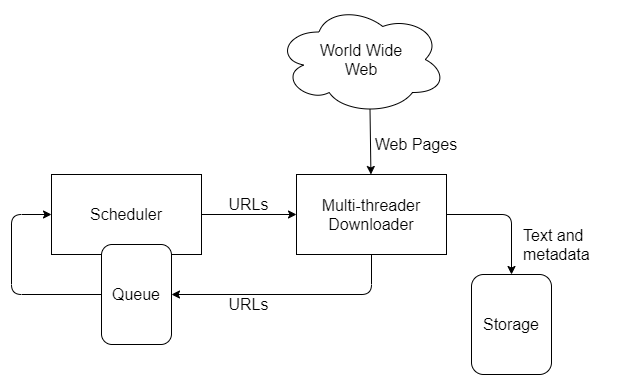
\includegraphics[keepaspectratio, width=12cm]{gambar/Arsitektur_Webcrawler}
	\caption{\emph{High Level Architecture of Web Crawler}~\cite{castillo2005effective}}
	\label{gambar:architecture_webcrawler}
\end{figure}

